\RequirePackage{scrlfile}
\ReplacePackage{scrpage2}{scrlayer-scrpage}

\documentclass[paper=a4,12pt,pointlessnumbers,twoside]{scrreprt}
\usepackage[automark]{scrlayer-scrpage} 
% Encoding UTF8
\usepackage[utf8]{inputenc}
% 8 Bit Aufloesung der Buchstaben
\usepackage[T1]{fontenc}
% Seitenraender
\usepackage[scale=0.72]{geometry}
% Spracheinstellungen
\usepackage[english, naustrian]{babel} % your native language must be the last one!!
% erweiterte Farbenpalette
\usepackage[dvipsnames, table]{xcolor}
% Abbildungen
\usepackage{graphicx}
% Tabellen (erweitert)
\usepackage{tabularx}
% Mathematikpakete!
\usepackage{amsmath,amssymb}							
\usepackage{mathtools}	
% PDF Einbindung (zB Datenblaetter)
\usepackage{pdfpages}
% Source Code Einbindung, Setup siehe:
% http://en.wikibooks.org/wiki/LaTeX/Source_Code_Listings									
\usepackage{listings,scrhack} %scrhack vermeidet Umschaltung auf KOMA Floats..			
			
\usepackage{verbatim}
\usepackage{textcomp}

\usepackage{bookmark}

\usepackage{eurosym}
\usepackage{lscape}
% Diplomarbeitsspezifisches Package etdipa

\usepackage{keyval}
\usepackage{caption}

%% Subfigures
\usepackage[lofdepth]{subfig}

\usepackage{import}

\usepackage{nameref}
\usepackage{arrayjob}
% folowing  must be in this order
\usepackage{varioref}
% \usepackage[colorlinks=true,
% 			linkcolor=black,
% 			citecolor=black,
% 			bookmarks=true,
% 			urlcolor=black,
% 			bookmarksopen=true]{hyperref}
\usepackage{cleveref}
\usepackage{float}
\usepackage{rotating}
\usepackage{longtable}
%\usepackage[allfiguresdraft]{draftfigure}
\usepackage{enumitem}
\usepackage{multicol}
\usepackage{array}

\usepackage{fancyvrb} %Fancy Code-Layout
\usepackage{xparse}

\usepackage{acronym}

\usepackage{algpseudocode, algorithm}

\newcolumntype{L}[1]{>{\raggedright\let\newline\\\arraybackslash\hspace{0pt}}p{#1}}

\RedeclareSectionCommand[beforeskip=0pt]{chapter}

\pdfcompresslevel=9 
\pdfobjcompresslevel=9

\begin{document}
\chapter{Die Hardware}
\section{Versorgung und Einschaltung}

Es ist vorgesehen, das Gerät mit 24V Gleichspannung zu betreiben.
Dafür ist eine Buchse links an der vorderen Seite des Gehäuses herausgeführt.
Um den Raspberry Pi zu starten, braucht das Gerät nur an den passenden Stecker angesteckt werden.

\section{Buchsen für die Sensorschnittstellen}

Datenblatt: \url{https://xonstorage.blob.core.windows.net/pdf/cixikefa_jh1712p4p_xonjuly20_12_link.pdf}\\[0.5cm]
Es sind 4 Buchsen des Typs JH1710S-4P an der Vorderseite des Geräts herausgeführt, jeder davon kann einen Sensor auslesen.

\subsection{Pinbelegung}
Die Stecker verfügen über 4 Pins (nummeriert von 1 bis 4), davon sind aber nur 3  belegt (24V DC Versorgung, 4-20mA Datenleitung, GND).

\begin{itemize}
    \item Pin 1: Versorgung 24V DC (rotes Kabel im Gerät)
    \item Pin 2: GND (schwarzes Kabel im Gerät)
    \item Pin 3: Datenleitung 4-20mA (weißes Kabel im Gerät)
    \item Pin 4: offen
\end{itemize}



\subsection{Nenndaten}

\begin{itemize}
    \item Nennstrom: 5A
    \item Nennspannung: 200V
\end{itemize}

\section{USB-Port}
Um die ausgewerteten Daten des Geräts speichern zu können, befindet sich auf der linken Seite des Geräts eine USB-Buchse.

\newpage
\begin{figure}[h]
    \centering
    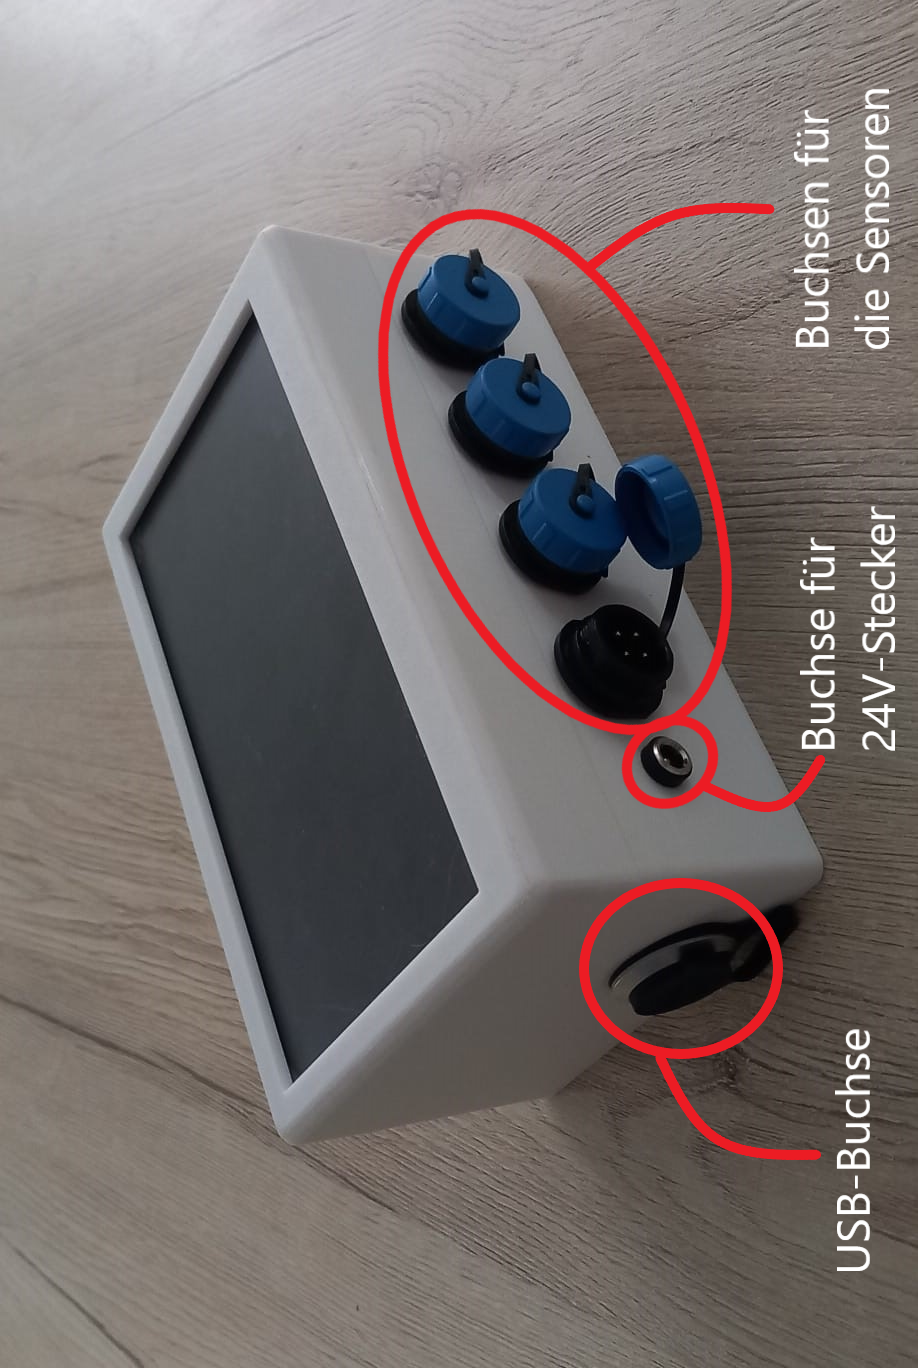
\includegraphics[width=0.9\linewidth]{Images/Gehause.bmp.png}
    \caption{Alle Buchsen des Gehäuses}
    \label{fig:Buchsen}
\end{figure}
\section{Schraubklemme zur Versorgung des Zusatzprints}
Die Schraubklemme zur Versorgung des Zusatzprints befindet sich auf der rechten Seite des Zusatzprints (Abb. \ref{fig:Zusatzprint}).

\section{Schraubklemmen für die 4-20mA Datenleitungen}
Der Zusatzprint kann bis zu 8 Sensoren auslesen. Die Leitungen werden dazu an die beiden Schraubklemmen auf der oberen Seite des Zusatzprints (Abb. \ref{fig:Zusatzprint}) angehängt.
Standardmäßig ist der erste ADC aktiviert und der zweite ADC deaktiviert.
Wenn mehr als 4 Sensoren eingelesen werden wollen, muss der zweite ADC softwaretechnisch erst aktiviert werden.

\section{Schraubklemme zur Versorgung der Sensoren}
Eine Schreibklemme, an der 24V Gleichspannung anliegen, befindet sich neben den Schraubklemmen für die Datenleitungen (Abb. \ref{fig:Zusatzprint}) und ist dazu gedacht, die Sensoren zu versorgen.\\
Es können in eine Öffnung mehrere Kabel gesteckt werden, wenn mehr als 4 Sensoren versorgt werden sollen.

\section{Schraubklemme um die Sensoren mit GND zu verbinden}
Die Schraubklemme, um die Sensoren mit GND zu verbinden, befindet sich neben der Schraubklemme für die Versorgung der Sensoren (Abb. \ref{fig:Zusatzprint}).\\
Auch hier können mehrere Kabel in eine Öffnung gesteckt werden.

\newpage
\begin{figure}[h]
    \centering
    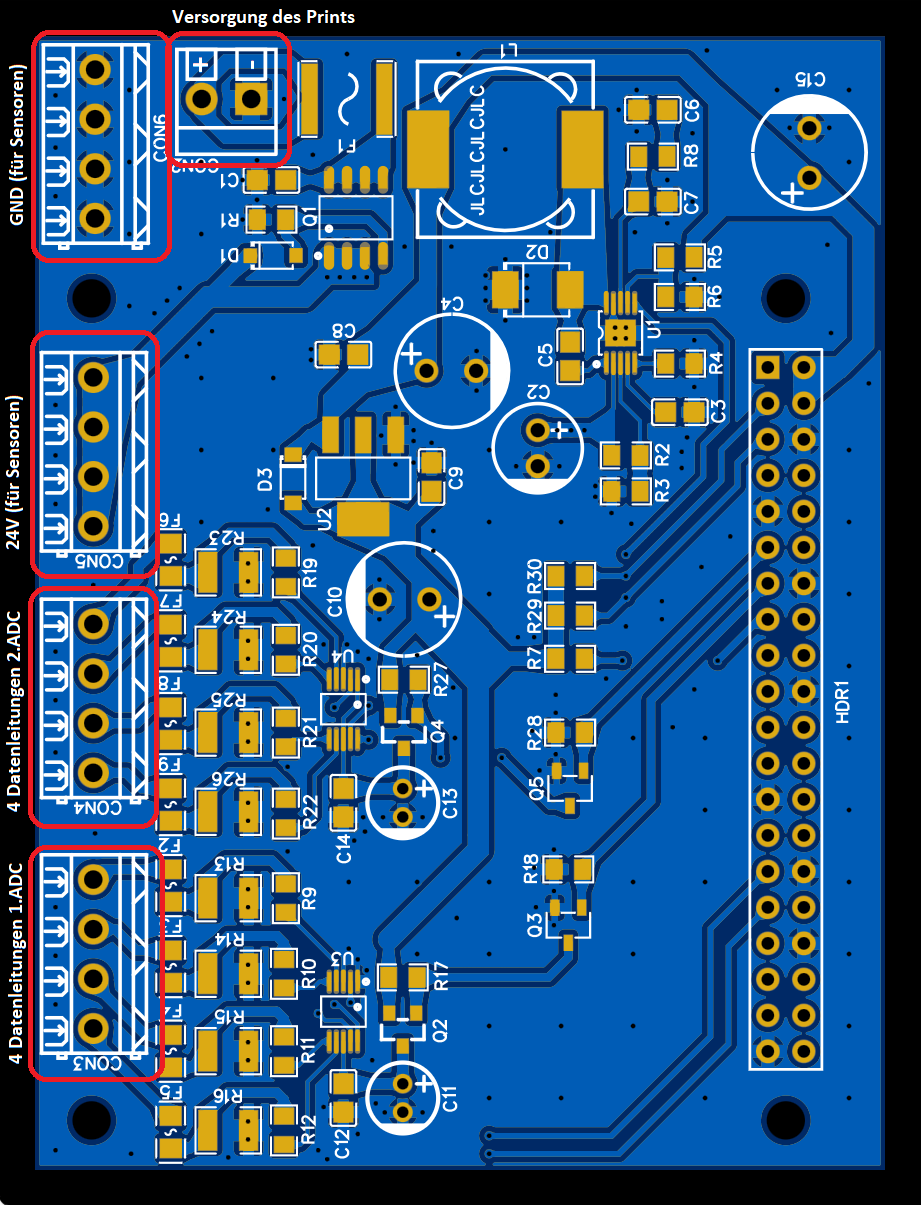
\includegraphics[width=1\linewidth]{Images/PCB1.PNG}
    \caption{Zusatzprint}
    \label{fig:Zusatzprint}
\end{figure}
\chapter{Das Web-Interface}

Das Web-Interface kann in einem Browser über folgende URL abgerufen werden: \verb|http://localhost:3001|.
Es ist wichtig, dass \verb|localhost| verwendet wird und nicht die IP des Docker-Containers, da 
Probleme mit der CORS-Policy entstehen können. Alle Graphen sind untereinander angeordnet; 
um die individuellen Kosten anzupassen, kann auf den jeweiligen Graphen geklickt werden, 
und im Eingabefeld können die Kosten in Cent eingegeben werden. Um die Datenbank verwalten zu können, 
wurde PHPmyAdmin verwendet, welches auf folgender URL abgerufen werden kann: \verb|http://localhost:81|.
Die Anmeldedaten für die Datenbank lauten: 
\\
User: \verb|root|
\\
Password: \verb|RZp7z1FNp3atzHth|
\\
Datenbank: \verb|sensor|

\section{Mögliche Fehlerquellen}

Sollte das RaspberryPi neu gestartet werden, kann es vorkommen, dass sich die IP-Adresse der Datenbank
innerhalb des Docker Containers verändert hat. Im root-Verzeichnis des Projekts (\verb|~/Documents/diplomarbeit/|) befindet sich ein 
Skript namens \verb|init_db_ip.sh|. Dieses aktualisiert die IP-Adresse der Datenbank im Server. 
Es sollten folgende Schritte hintereinander ausgeführt werden, um die API (den Server) neu zu starten:
\\
\\
\verb|$> cd ~/Documents/diplomarbeit|
\\
\verb|$> ./init_db_ip.sh|
\\
\verb|$> sudo docker stop diplomarbeit_api|
\\
\verb|$> sudo docker remove diplomarbeit_api|
\\
\verb|$> cd web/|
\\
\verb|$> sudo docker compose up -d|
\\
\\
Falls die Datenbank noch nicht läuft, sollte das Docker Compose projekt angestartet werden:
\\
\verb|$> cd ~/Documents/diplomarbeit/web|
\\
\verb|$> sudo docker compose up -d|
\\
\\
Ob jeder Container erfolgreich läuft, kann mit folgendem Befehl überprüft werden:
\\
\verb|$> sudo docker ps -a|
\\
\\
Sollten keine Graphen angezeigt werden, kann über folgendem Befehl bei der API auf Fehlernachrichten überprüft werden:
\\
\verb|$> sudo docker logs diplomarbeit_api|



\end{document}
